\begin{remark}[Soundness over all databases is too strong for \texttt{rate}]
Even on $\mathcal{C}_{\mathrm{warm}}$, \texttt{rate} is not $\varepsilon$-sound over all
databases for any $\varepsilon<1$ under relative error: if the whole increase falls
between the last sample before the window and the first sample inside it, one system
returns $0$ while the other counts the delta. Useful bounds must therefore restrict the
data class, e.g.\ to counters whose per-scrape increments vary by at most a factor
$\beta$, and state $\varepsilon$ as a function of $\beta$, the scrape interval $s$ and
the window $w$. Figure~\ref{fig:rate-error} shows how the error shrinks as $\Delta$ grows
relative to the scrape interval.
\end{remark}

\begin{figure}[htbp]\centering
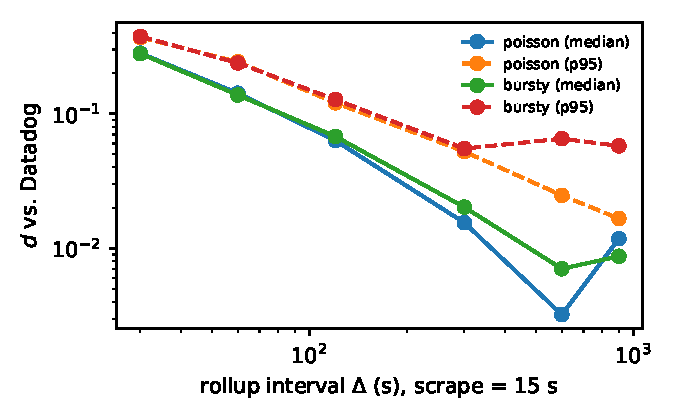
\includegraphics[width=0.6\linewidth]{figures/rate_error_vs_window}
\caption{Error of \texttt{rate()} against Datadog as the rollup interval grows, at a
$15$\,s scrape interval. \texttt{rate} is the only candidate whose error depends on the
data.}
\label{fig:rate-error}
\end{figure}
